\section{ASL Finger Spelling with ConvNets}

% self.layers = nn.Sequential(
            
% #? first convolutional layer
% nn.Conv2d(1, 32, kernel_size=3, stride=1),
% nn.ReLU(),
% nn.MaxPool2d(kernel_size=2, stride=2),

% #? second convolutional layer
% nn.Conv2d(32, 64, kernel_size=3, stride=1),
% nn.ReLU(),
% nn.MaxPool2d(kernel_size=2, stride=2),

% #? third convolutional layer
% nn.Conv2d(64, 64, kernel_size=3, stride=1),
% nn.ReLU(),
% nn.MaxPool2d(kernel_size=2, stride=2),

% #? flatten the output
% nn.Flatten(),

% #? 128-neurons linear layer
% nn.Linear(64, 128),

% #? relu activation
% nn.ReLU(),

% #? output layer with <classes> neurons
% nn.Linear(128, classes)
% )

\begin{problem}
  What is a kernel?
  \begin{answer}
    A kernel is a window (matrix) of values that we
    slide over the input image to produce a feature map.
    Features can be lines, edges, corners, etc.
  \end{answer}
\end{problem}

\begin{problem}
  What is pooling?
  \begin{answer}
    Pooling is a technique used to reduce the spatial dimensions of a convolutional layer.
    This can take various forms, such as max-pooling, average-pooling, etc,
    where we take the maximum or average value of each window of values.
    The stride of the pooling layer determines how much we move the window
    over the input tensor after each pooling operation.
  \end{answer}
\end{problem}

\newpage
\begin{problem}
  How does the size of the image change as it passes through the network?
  \begin{answer}
    \begin{enumarabic}
      \item The first convolutional layer has $32$ output channels and a kernel size of $3$,
        followed by a \verb|ReLU| layer and a max-pooling layer with a kernel size of $2$.
        \begin{enumroman}
          \item \verb|nn.Conv2d(1, 32, kernel_size=3, stride=1)|
            \[ (28 \times 28 \times 1) \mapsto (26 \times 26 \times 32) \]
          \item \verb|nn.ReLU()|
            \[ (26 \times 26 \times 32) \mapsto (26 \times 26 \times 32) \]
          \item \verb|nn.MaxPool2d(kernel_size=2, stride=2)|
            \[ (26 \times 26 \times 32) \mapsto (13 \times 13 \times 32) \]
        \end{enumroman}
      \item The second convolutional layer has $32$ input channels and $64$ output channels,
        with a kernel size of $3$, followed by a \verb|ReLU| layer and a max-pooling layer with a kernel size of $2$.
        \begin{enumroman}
          \item \verb|nn.Conv2d(32, 64, kernel_size=3, stride=1)|
            \[ (13 \times 13 \times 32) \mapsto (11 \times 11 \times 64) \]
          \item \verb|nn.ReLU()|
            \[ (11 \times 11 \times 64) \mapsto (11 \times 11 \times 64) \]
          \item \verb|nn.MaxPool2d(kernel_size=2, stride=2)|
            \[ (11 \times 11 \times 64) \mapsto (5 \times 5 \times 64) \]
        \end{enumroman}
      \item The third convolutional layer has $64$ input channels and $64$ output channels,
        with a kernel size of $3$, followed by a \verb|ReLU| layer and a max-pooling layer with a kernel size of $2$.
        \begin{enumroman}
          \item \verb|nn.Conv2d(64, 64, kernel_size=3, stride=1)|
            \[ (5 \times 5 \times 64) \mapsto (3 \times 3 \times 64) \]
          \item \verb|nn.ReLU()|
            \[ (3 \times 3 \times 64) \mapsto (3 \times 3 \times 64) \]
          \item \verb|nn.MaxPool2d(kernel_size=2, stride=2)|
            \[ (3 \times 3 \times 64) \mapsto (1 \times 1 \times 64) \]
        \end{enumroman}
      \item We then have a \verb|nn.Flatten()| layer that flattens the vector.
        \[ (1 \times 1 \times 64) \mapsto (64) \]
      \item We then have a \verb|nn.Linear(64, 128)| layer that outputs.
        \[ (64) \mapsto (128) \]
      \item We then have a \verb|nn.ReLU()| layer (activation function,
      does not change the size of the tensor) followed by a \verb|nn.Linear(128, classes)|
      layer that outputs final predictions.
        \[ (128) \mapsto (\text{classes}) \]
    \end{enumarabic}
  \end{answer}
\end{problem}

\newpage
\begin{problem}
  Run the program.
  How is the network behaving after one epoch of training?
  Report this based on the accuracy, the precision, and the recall for each of the letters.
  Include screenshots of your results.
\end{problem}

\begin{answer}
  The network has an overall accuracy of $0.95$, with slightly better \verb|F1| scores
  for certain letters and slightly worse for others.

  
  
\end{answer}
\begin{table}[H]
  \centering
  \begin{tabular}{|c|c|c|c|c|}
  \midrule
  \textbf{Class} & \textbf{Precision} & \textbf{Recall} & \textbf{F1-Score} & \textbf{Support} \\
  \midrule
  $0$              & $1.00$             & $0.90$          & $0.95$            & $331$           \\
  \midrule
  $1$              & $1.00$             & $0.89$          & $0.94$            & $432$           \\
  \midrule
  $2$              & $0.99$             & $1.00$          & $0.99$            & $310$           \\
  \midrule
  $3$              & $0.99$             & $0.92$          & $0.96$            & $245$           \\
  \midrule
  $4$              & $0.90$             & $0.98$          & $0.94$            & $498$           \\
  \midrule
  $5$              & $0.83$             & $1.00$          & $0.91$            & $247$           \\
  \midrule
  \end{tabular}
  \caption{Accuracy and F1 scores for each letter.}
  \label{tab:accuracy-f1}
\end{table}

\begin{table}[h]
  \centering
  \begin{tabular}{|c|c|c|c|c|c|}
  \midrule
  297 & 0   & 0   & 1   & 33  & 0   \\ \midrule
  0   & 384 & 0   & 0   & 0   & 48  \\ \midrule
  0   & 0   & 310 & 0   & 0   & 0   \\ \midrule
  0   & 0   & 0   & 226 & 19  & 0   \\ \midrule
  0   & 0   & 4   & 1   & 490 & 3   \\ \midrule
  0   & 0   & 0   & 0   & 0   & 247 \\ \midrule
  \end{tabular}
  \caption{Confusion Matrix}
  \label{tab:confusion-matrix}
\end{table}

\textbf{Screenshots}
\begin{figure}[H]
  %  minipages
  \centering
  \begin{minipage}[b]{0.59\textwidth}
    \centering
    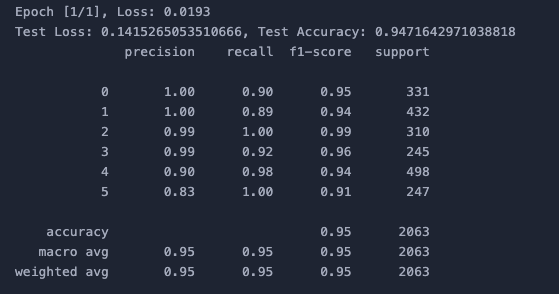
\includegraphics[width=0.9\textwidth]{figures/2-accuracy.png}
    \caption{ASL Finger Spelling}
    \label{fig:asl-fs-1}
  \end{minipage}
  \hfill
  \begin{minipage}[b]{0.39\textwidth}
    \centering
    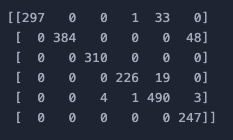
\includegraphics[width=0.9\textwidth]{figures/2-confusion.png}
    \caption{ASL Finger Spelling}
    \label{fig:asl-fs-2}
  \end{minipage}
\end{figure}
